\documentclass[11pt]{article}

\usepackage[utf8]{inputenc}
\usepackage[margin=1in]{geometry}  % Adjust page margins
\usepackage{graphicx}              % For including images (PDF, PNG, JPG)
\usepackage[inkscapelatex=false]{svg}
\usepackage{listings}              % For including code
\usepackage{xcolor}                % For custom colors
\usepackage{hyperref}              % For hyperlinks in the PDF
\usepackage{amsmath, amssymb, amsthm} % For math symbols and environments
\usepackage{mathrsfs}
\usepackage{enumitem}
\geometry{a4paper, margin=1in} % Set margin to 1 inch
\usepackage{fancyhdr} % For header and footer
\usepackage{hyperref} % For clickable links in the PDF
\usepackage{array} % For table column formatting
\usepackage{times} % Uses Times font for the text
\usepackage{float}
\usepackage{multirow}
\usepackage{booktabs}


\title{CMOR 421/521 Assignment 2: OpenMP}
\author{Yuhao Liu}
\date{\today}

% --------------------------------------------------------------------------------
% Customize the appearance of code listings (for C++ syntax).
% --------------------------------------------------------------------------------
\lstdefinestyle{C++Style}{
    language=C++,
    basicstyle=\small\ttfamily,
    keywordstyle=\color{blue}\bfseries,
    commentstyle=\color{gray},
    stringstyle=\color{magenta},
    numbers=left,
    numberstyle=\tiny,
    stepnumber=1,
    breaklines=true,
    tabsize=4,
    showstringspaces=false
}

% If you store SVG images in a subfolder, specify the path here. 
% e.g.: \svgpath{{../images/}}
\svgpath{{./}}

\begin{document}

\maketitle

\tableofcontents
\bigskip

\newpage

\section{Directory Structure}
Below is my file organization for this assignment. 
My final zip file follows this structure ( \texttt{docs/} for LaTeX, \texttt{src/} for source files, and \texttt{include/} for header files):

\begin{figure}[H]
    \centering
    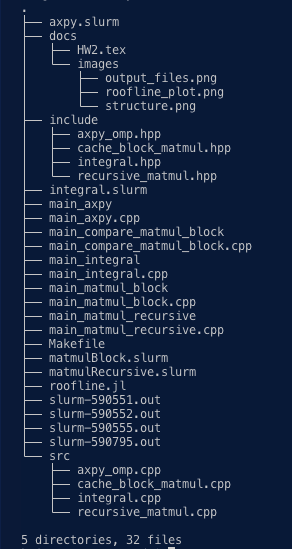
\includegraphics[width=0.3\linewidth]{Assignments/HW2/docs/images/structure.png}
    \caption{structure}
    \label{fig:structure}
\end{figure}

\begin{itemize}
    \item The \verb|main_axpy.cpp|, \verb|main_matmul_block.cpp|, \verb|main_compare_matmul_block.cpp|, \verb|main_matmul_recursive.cpp|, and \verb|main_integral.cpp| are include the \verb|main| functions for the parallelized \verb|AXPY|, \verb|Cache Block Matrix Multiplication|, \verb|Recursive Matrix Multiplication|, and \verb|Integral Pi|
    \item The \verb|roofline.jl| plot the roofline figure, and calculate the percentage of peak performance.
    \item The \verb|main_axpy|, \verb|main_matmul_block|, \verb|main_matmul_recursive|, \verb|main_compare_matmul_block|, and \verb|main_integral| are execution file which already by compiled. You can directly run these file in your local computer as long as you have 16 threads in your computer. If you want to compile each of them, you can using the command in the next section.
    \item The \verb|axpy.slurm|, \verb|matmulBlock.slurm|, \verb|matmulRecursive.slurm|, and \verb|integral.slurm| are script file to help run the execution file in NOTXs. I already set 16 cores for each of task. But its were made by my personal account. You can directly using the command in the next section to run the file after changed the account.
    \item The folder \texttt{docs/} is to store the Latex file and images.
    \item The folder \texttt{include/} is the place for \verb|.hpp| files. The \verb|axpy_omp.hpp|, \verb|cache_block_matmul.hpp|, \verb|recursive_matmul.hpp|, and \verb|integral.hpp| are in there.
    \item The folder \texttt{src/} is the place for \verb|axpy_omp.cpp|, \verb|cache_block_matmul.cpp|, \verb|recursive_matmul.cpp|, and \verb|integral.cpp|  which are used to implemented all different methods for matrix transpose, matrix multiplication, and the timing analysis functions.


\end{itemize}

\newpage

\section{How to Build and Run the Code (In NOTXs)}
\label{sec:build_run}
\begin{itemize}
    \item \textbf{Build Instructions:} 
        \begin{itemize}
            \item For all executable file, you can directly using
            \begin{verbatim}
                make
            \end{verbatim}
            to build all executable file.
            
        \end{itemize}
    \item \textbf{Running Instructions:} 
        Once you build the execution file, it will appear as driver files. You can use the following command to run the code in NOTXs:
        \begin{verbatim}
            sbatch axpy.slurm
            sbatch matmulBlock.slurm
            sbatch matmulRecursive.slurm
            sbatch integral.slurm
        \end{verbatim}
    \item  \textbf{Execution: }
        When you execute the program, in the terminal you can see the output file in the drive folder:
        \begin{figure}[H]
            \centering
            
\includegraphics[width=0.5\linewidth]{Assignments/HW2/docs/images/output_files.png}
            \caption{Output files}
            \label{fig:Output files}
        \end{figure}
        These output file will storage the output for each task.

        If you want to clean all executable files, using
        \begin{verbatim}
            make clean
        \end{verbatim}
\end{itemize}

\newpage

\section{Analysis}
In this section, I will show you the analysis for these results. All the parallel \textit{efficiency} for strong scaling, I followed the Amdahl's law:
\begin{equation*}
    E(n) = \frac{S(n)}{n}
\end{equation*}
where 
\begin{equation*}
    S(n) = \frac{T(1)}{T(n)}
\end{equation*}

For the weak scaling, I only compute the parallel speed-up with
\begin{equation*}
    S(n) = \frac{T(1)}{T(n)}
\end{equation*}

\subsection{AXPY}
For the \verb|AXPY| method in \verb|version_1| and \verb|version_2|, from the following table (Strong Scaling):
\begin{table}[H]
\centering
\begin{tabular}{|c|c|c|c|}
\hline
\textbf{AXPY Version} & \textbf{Threads} & \textbf{Runtime} & \textbf{Efficiency} \\ \hline
\multirow{5}{*}{Version 1} 
& 1  & 5.94938  & 1        \\ \cline{2-4}
& 2  & 1.72952  & 1.71995  \\ \cline{2-4}
& 4  & 1.26784  & 1.17313  \\ \cline{2-4}
& 8  & 1.16535  & 0.638155 \\ \cline{2-4}
& 16 & 1.84623  & 0.201403 \\ \hline
\multirow{5}{*}{Version 2} 
& 1  & 2.67886  & 1        \\ \cline{2-4}
& 2  & 1.45018  & 0.92363  \\ \cline{2-4}
& 4  & 0.746254 & 0.897436 \\ \cline{2-4}
& 8  & 0.464915 & 0.720256 \\ \cline{2-4}
& 16 & 0.432303 & 0.387295 \\ \hline
\end{tabular}
\caption{Runtime and Efficiency of AXPY Versions}
\label{tab:AXPY}
\end{table}
We can find that for \verb|version_1|, after we increased the number of threads, the runtime without keeping decreasing instead of increasing, like \verb|Threads = 16|. The efficiency increased at first and then decreased. On the other hands, we can see that the \verb|version_2| is more general since it's runtime keeping decreased and the efficiency reduced normally. 

\newpage
\subsubsection{Strong and Weak scaling}
In this part, I will perform strong and weak scaling studies for up to 16 threads. The reults table is as following:
\begin{table}[H]
\centering
\resizebox{\textwidth}{!}{
\begin{tabular}{|c|c|c|c|c|}
\hline
\textbf{Scaling Experiment} & \textbf{AXPY Version} & \textbf{Threads} & \textbf{Runtime (s)} & \textbf{Efficiency (Speed Up)} \\ \hline
\multirow{10}{*}{Strong Scaling} 
& \multirow{5}{*}{Version 1} 
& 1  & 5.68555  & 1.000000 \\ \cline{3-5}
& & 2  & 2.45827  & 1.156410 \\ \cline{3-5}
& & 4  & 1.88886  & 0.752513 \\ \cline{3-5}
& & 8  & 2.24959  & 0.315922 \\ \cline{3-5}
& & 16 & 1.68469  & 0.210928 \\ \cline{2-5}

& \multirow{5}{*}{Version 2} 
& 1  & 3.13006  & 1.000000 \\ \cline{3-5}
& & 2  & 1.55607  & 1.005760 \\ \cline{3-5}
& & 4  & 0.849503 & 0.921146 \\ \cline{3-5}
& & 8  & 0.509333 & 0.768178 \\ \cline{3-5}
& & 16 & 0.305709 & 0.639919 \\ \hline

\multirow{10}{*}{Weak Scaling} 
& \multirow{5}{*}{Version 1} 
& 1  & 0.360786 & 1.000000 \\ \cline{3-5}
& & 2  & 0.813838 & 0.443314 \\ \cline{3-5}
& & 4  & 2.11619  & 0.170489 \\ \cline{3-5}
& & 8  & 6.72802  & 0.053624 \\ \cline{3-5}
& & 16 & 21.7201  & 0.016611 \\ \cline{2-5}

& \multirow{5}{*}{Version 2} 
& 1  & 0.190484 & 1.000000 \\ \cline{3-5}
& & 2  & 0.241768 & 0.787878 \\ \cline{3-5}
& & 4  & 0.246050 & 0.774168 \\ \cline{3-5}
& & 8  & 0.294072 & 0.647746 \\ \cline{3-5}
& & 16 & 0.406239 & 0.468897 \\ \hline
\end{tabular}}
\caption{Strong and Weak Scaling Results for AXPY Operation}
\label{tab:axpy_scaling}
\end{table}

From the table \ref{tab:axpy_scaling}, we can find the result of runtime and parallel efficiency for each type of scaling. 

I think \textbf{version 2} clearly scales better than Version 1 in both the strong‐scaling and weak‐scaling experiments. 
\begin{itemize}
    \item In strong scaling, version 2 starts at about 3.13s (1 thread) and goes down to about 0.31 s (16 threads). That is roughly a 10× speedup, with an efficiency of around 64\% on 16 threads. Version 1, on the other hand, shows a speedup of only about 3.4× at 16threads (down from 5.69s to 1.68s), for an efficiency around 21\%. 
    \item In weak scaling, the ideal is to keep runtime nearly constant as you add threads and proportionally increase the problem size. Version 2 remains under a second up to 16 threads (0.41s at 16threads), while Version 1 increases to over 21s at 16 threads. Accordingly, Version 2’s efficiency in the weak‐scaling section (0.47 at 16 threads) is substantially higher than Version 1’s (0.011 at 16 threads).
\end{itemize}

\newpage
\subsubsection{Roofline Model(CMOR 521)}
The figure of Roofline is:
\begin{figure}[H]
        \centering
        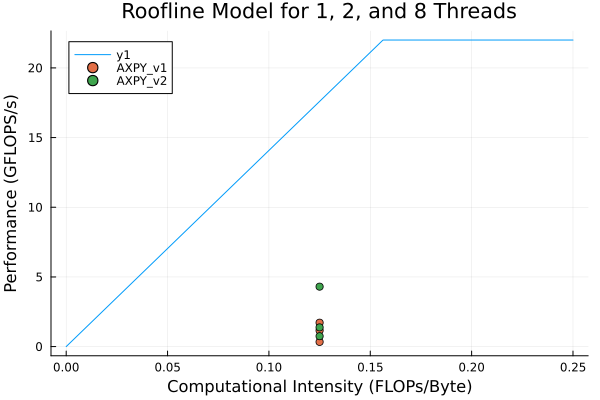
\includegraphics[width=0.75\linewidth]{Assignments/HW2/docs/images/roofline_plot.png}
        \caption{Roofline Model}
        \label{fig:Roofline Model}
    \end{figure}
The percentage of peak performance do you achieve for each case are as following:
\begin{table}[H]
\centering
\begin{tabular}{ccc}
\toprule
\textbf{Threads} & \textbf{AXPY Version} & \textbf{Performance (\% of Peak)} \\
\midrule
1 & v1 & 1.53\% \\
2 & v1 & 2.63\% \\
8 & v1 & 0.98\% \\
1 & v2 & 3.39\% \\
2 & v2 & 3.13\% \\
8 & v2 & 2.44\% \\
\bottomrule
\end{tabular}
\caption{Achieved performance compared to theoretical peak performance}
\label{tab:performance}
\end{table}

\newpage

\subsection{Matrix Multiplication (Cache Block)}

\subsubsection{Compare "\#omp parallel for" with "\#omp parallel for collapse(...)"}
In this part, firstly, we need to compare the "\#omp parallel for" with "\#omp parallel for collapse(...)" and determined the optimal collapse parameter. Since the cache block matrix method can only stand for 2 or 3 collapse parameter, and the result for these three different parallelization way in the following table:
\begin{table}[H]
\centering
\begin{tabular}{|c|c|c|c|c|}
\hline
\textbf{Version} & \textbf{Threads} & \textbf{Matrix Size} & \textbf{Runtime} & \textbf{Efficiency} \\ \hline
\multirow{5}{*}{MatMul Standard} 
& 1  & \multirow{5}{*}{2048} & 27.06997 & 1.00000 \\ \cline{2-2} \cline{4-5}
& 2  & & 13.48462 & 1.00373 \\ \cline{2-2} \cline{4-5}
& 4  & & 6.76744  & 1.00001 \\ \cline{2-2} \cline{4-5}
& 8  & & 3.89171  & 0.86947 \\ \cline{2-2} \cline{4-5}
& 16 & & 4.00292  & 0.42266 \\ \hline
\multirow{5}{*}{MatMul Collapse(2)} 
& 1  & \multirow{5}{*}{2048} & 28.53727 & 1.00000 \\ \cline{2-2} \cline{4-5}
& 2  & & 13.47711 & 1.05873 \\ \cline{2-2} \cline{4-5}
& 4  & & 6.76001  & 1.05537 \\ \cline{2-2} \cline{4-5}
& 8  & & 3.91194  & 0.91186 \\ \cline{2-2} \cline{4-5}
& 16 & & 4.01510  & 0.44422 \\ \hline
\multirow{5}{*}{MatMul Collapse(3)} 
& 1  & \multirow{5}{*}{2048} & 27.69317 & 1.00000 \\ \cline{2-2} \cline{4-5}
& 2  & & 13.52404 & 1.02385 \\ \cline{2-2} \cline{4-5}
& 4  & & 6.78140  & 1.02092 \\ \cline{2-2} \cline{4-5}
& 8  & & 3.86833  & 0.89487 \\ \cline{2-2} \cline{4-5}
& 16 & & 3.78207  & 0.45764 \\ \hline
\end{tabular}
\caption{Strong Scaling Experiment (Matrix Size = 2048 $\times$ 2048)}
\label{tab:matmul_scaling}
\end{table}

Based on the results, collapse(3) appears to be the optimal variant. Since all three variants have similar runtimes with one thread (Standard: 27.07s, collapse(2): 28.54s, collapse(3): 27.69s), so the difference isn’t significant when parallelism isn’t leveraged. At 2 and 4 threads, all versions achieve nearly identical performance, with efficiencies around or slightly above 1 (even a bit over 1 can happen because of improved cache reuse or other micro-architectural effects). As the thread count increases, the differences become clearer:
\begin{itemize}
    \item With 8 threads, Collapse(3) shows the lowest runtime (3.86833s) compared to Standard (3.89171s) and Collapse(2) (3.91194s).
    \item At 16 threads, Collapse(3) delivers a runtime of 3.78207s and an efficiency of 0.45764, which is noticeably better than Standard (4.00292s, 0.42266 efficiency) and Collapse(2) (4.01510s, 0.44422 efficiency).
\end{itemize}

Therefore collapsing three loops provides a larger iteration space.

\newpage
\subsubsection{Strong and Weak scaling}
In this part, I will perform strong and weak scaling studies for up to 16 threads. The reults table is as following:
\begin{table}[H]
\centering
\resizebox{\textwidth}{!}{
\begin{tabular}{|c|c|c|c|c|c|}
\hline
\textbf{Experiment} & \textbf{Version} & \textbf{Threads} & \textbf{Matrix Size} & \textbf{Runtime (s)} & \textbf{Efficiency (Speed Up)} \\ \hline
\multirow{10}{*}{Strong Scaling} 
& \multirow{5}{*}{MatMul Standard} 
& 1 & 2048 & 27.10687 & 1.00000 \\ \cline{3-6}
& & 2 & 2048 & 13.54723 & 1.00046 \\ \cline{3-6}
& & 4 & 2048 & 6.76382 & 1.00191 \\ \cline{3-6}
& & 8 & 2048 & 3.83429 & 0.88370 \\ \cline{3-6}
& & 16 & 2048 & 3.85602 & 0.43936 \\ \cline{2-6}

& \multirow{5}{*}{MatMul Collapse(2)} 
& 1 & 2048 & 28.20344 & 1.00000 \\ \cline{3-6}
& & 2 & 2048 & 14.06791 & 1.00240 \\ \cline{3-6}
& & 4 & 2048 & 7.03822 & 1.00180 \\ \cline{3-6}
& & 8 & 2048 & 4.14558 & 0.85041 \\ \cline{3-6}
& & 16 & 2048 & 4.28617 & 0.41126 \\ \hline

\multirow{10}{*}{Weak Scaling} 
& \multirow{5}{*}{MatMul Standard} 
& 1 & 128 & 0.00623 & 1.00000 \\ \cline{3-6}
& & 2 & 256 & 0.02621 & 0.11878 \\ \cline{3-6}
& & 4 & 512 & 0.10443 & 0.01490 \\ \cline{3-6}
& & 8 & 1024 & 0.44713 & 0.00174 \\ \cline{3-6}
& & 16 & 2048 & 3.84999 & 0.00010 \\ \cline{2-6}

& \multirow{5}{*}{MatMul Collapse(2)} 
& 1 & 128 & 0.00677 & 1.00000 \\ \cline{3-6}
& & 2 & 256 & 0.02709 & 0.12497 \\ \cline{3-6}
& & 4 & 512 & 0.10847 & 0.01560 \\ \cline{3-6}
& & 8 & 1024 & 0.50719 & 0.00167 \\ \cline{3-6}
& & 16 & 2048 & 4.29759 & 0.00010 \\ \hline
\end{tabular}}
\caption{Strong and Weak Scaling Experiments for Matrix Multiplication}
\label{tab:matmul_scaling}
\end{table}


\subsection{Recursive Matrix Multiplication}

In this part, I will perform strong and weak scaling studies for up to 16 threads. The reults table is as following:
\begin{table}[H]
\centering
\resizebox{\textwidth}{!}{
\begin{tabular}{|c|c|c|c|c|}
\hline
\textbf{Scaling Experiment} & \textbf{Threads} & \textbf{Matrix Size} & \textbf{Runtime (s)} & \textbf{Efficiency (Speed Up)} \\ \hline
\multirow{5}{*}{Strong Scaling} 
& 1 & 2048 & 24.50431 & 1.00000 \\ \cline{2-5}
& 2 & 2048 & 12.29185 & 0.99677 \\ \cline{2-5}
& 4 & 2048 & 6.47467  & 0.94616 \\ \cline{2-5}
& 8 & 2048 & 3.93354  & 0.77870 \\ \cline{2-5}
& 16 & 2048 & 3.63948 & 0.42081 \\ \hline

\multirow{5}{*}{Weak Scaling} 
& 1 & 128  & 0.00589  & 1.00000 \\ \cline{2-5}
& 2 & 256  & 0.02456  & 0.23989 \\ \cline{2-5}
& 4 & 512  & 0.10145  & 0.05806 \\ \cline{2-5}
& 8 & 1024 & 0.48898  & 0.01205 \\ \cline{2-5}
& 16 & 2048 & 3.64802 & 0.00161 \\ \hline
\end{tabular}}
\caption{Recursive Matrix Multiplication: Strong and Weak Scaling Results}
\label{tab:recursive_matmul_scaling}
\end{table}

\newpage
\subsection{(For CMOR 521)  Integral Pi}
In this part, I re-implement the integration code used in class using atomic operations and compared the performance of atomic operations to the reduction-based implementation by performing a strong scaling study for each implementation.

This part is the integration code used in class using atomic operations
\begin{lstlisting}[style=C++Style]
// Function that computes pi using atomic updates
double integral_atomic(int num_steps) {
    double step = 1.0 / num_steps;
    double sum = 0.0;
    #pragma omp parallel for
    for (int i = 0; i < num_steps; i++) {
        double x = (i + 0.5) * step;
        double temp = 4.0 / (1.0 + x * x);
        #pragma omp atomic
        sum += temp;
    }
    return step * sum;
}
\end{lstlisting}

This part is the integration code with the reduction-based implementation
\begin{lstlisting}[style=C++Style]
// Function that computes pi using the reduction clause
double integral_reduction(int num_steps) {
    double step = 1.0 / num_steps;
    double sum = 0.0;
    #pragma omp parallel for reduction(+:sum)
    for (int i = 0; i < num_steps; i++) {
        double x = (i + 0.5) * step;
        sum += 4.0 / (1.0 + x * x);
    }
    return step * sum;
}
\end{lstlisting}

The strong scaling result table is as following:

\begin{table}[H]
\centering
\begin{tabular}{|c|c|c|c|c|c|}
\hline
\textbf{Implementation} & \textbf{Threads} & \textbf{Time (s)} & \textbf{Speedup} & \textbf{Efficiency} & \textbf{Pi} \\ \hline
\multirow{5}{*}{Atomic}
& 1 & 0.964693 & 1.000000 & 1.000000 & 3.141593 \\ \cline{2-6}
& 2 & 5.435353 & 0.177485 & 0.088742 & 3.141593 \\ \cline{2-6}
& 4 & 6.622583 & 0.145667 & 0.036417 & 3.141593 \\ \cline{2-6}
& 8 & 6.744995 & 0.143024 & 0.017878 & 3.141593 \\ \cline{2-6}
& 16 & 5.788789 & 0.166649 & 0.010416 & 3.141593 \\ \hline
\multirow{5}{*}{Reduction}
& 1 & 0.235411 & 1.000000 & 1.000000 & 3.141593 \\ \cline{2-6}
& 2 & 0.123600 & 1.904615 & 0.952307 & 3.141593 \\ \cline{2-6}
& 4 & 0.063234 & 3.722870 & 0.930718 & 3.141593 \\ \cline{2-6}
& 8 & 0.033579 & 7.010662 & 0.876333 & 3.141593 \\ \cline{2-6}
& 16 & 0.032575 & 7.226819 & 0.451676 & 3.141593 \\ \hline
\end{tabular}
\caption{Strong Scaling Study for PI Integration (num\_steps = 100,000,000)}
\label{tab:pi_scaling}
\end{table}

\end{document}